\newpage
\chapter{Introduction}

The report presents theoretical analysis and experimental simulation data associated with the operation of a wind turbine with variable pitch. Pitch control is an important element of wind turbine design. Pitch control is analogous to the coarse control on a microscope. It is meant to facilitate a regular rotation rate for the blades. A well-tuned pitch control system allows for better and cheaper design of the generator control system. 

The effect of both supply volt and load torque changes is on the open loop response of the pitch control system is simulated in this report using Matlab and Simulink. The effects of both these input are also discussed.


The open loop frequency response of the system is examined. The magnitude and phase characteristics of this response are plot on Bode, Nichols and Nyquist plots. How these plots and the open loop response allow inferring of closed loop characteristics is explained. The usefulness of these plot in design controllers for the system is also considered in Figure~\ref{VbStep}.

\begin{figure}[htp]
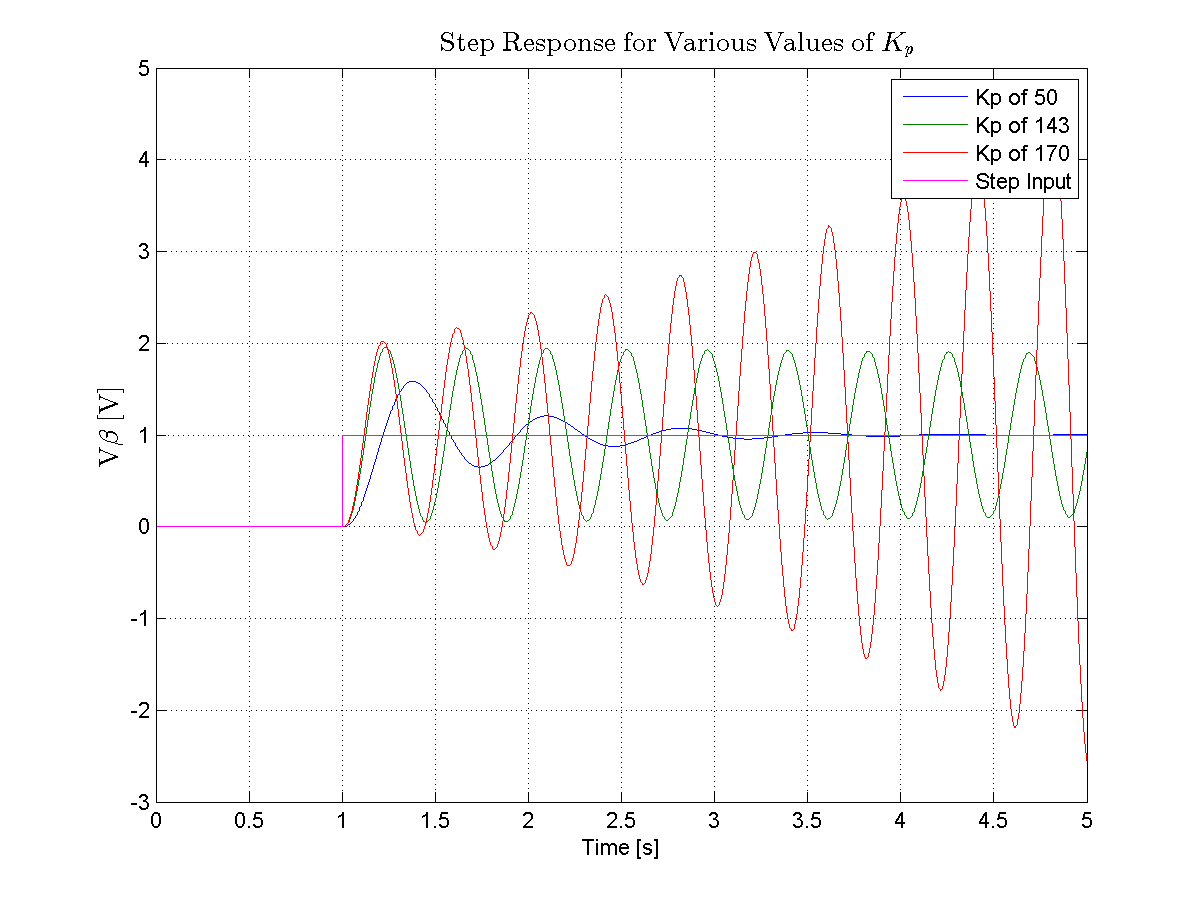
\includegraphics[width=\textwidth]{./img/StepResponseVb}
\caption{Step Response Vc}
\label{VbStep}
\end{figure}

The effect of adding a proportional controller and a phase lead controller to the turbine system is demonstrated. Methods used to optimize these controllers for various steady state and transient parameters are explored. The responses at various stages of the controller design process are simulated and compared.
Finally the limits of this model are acknowledge. Possible additions to increase the realism of this model are dealt with.

